\documentclass[../diploma.tex]{subfiles}
 
\begin{document}

WaveNet - это нейросетевая архитектура, вдохновлённая недавними достижениями в сфере нейросетевых авторегрессивных генеративных моделей, описывающих сложные распределения такие как картинки \cite{article:oord2016pixel} и текст \cite{article:jozefowicz2016exploring}. WaveNet - это модель для генерации аудио, основанная на PixelCNN \cite{article:oord2016conditional}.
В статье аудио сигналы получаются с помощью генеративной модели, оперирующей напрямую с необработанным цифровым сигналом, описывающим звуковую волну.

Совместная вероятность волны $x = \{ x_1, \dots, x_T \}$ описывается как произведение условных вероятностей уравнением \ref{eq:wave_distr}:

\begin{equation} \label{eq:wave_distr}
p(x) = \prod^{T}_{t=1}{} p(x_t|x_1, \dots, x_{t-1})
\end{equation}

Таким образом, каждая точка аудиосигнала $x_t$ зависит от всех предыдущих.

\begin{definition}
\textbf{Стеком} слоёв в нейросети будем называть последовательный набор слоёв со следующим свойством: выход каждого слоя передаётся в качестве входа к следующему за ним. В контексте данной работы мы будем чаще всего говорить о стеках свёрточных слоёв.
\end{definition}

\begin{definition}

В контексте свёрточных нейронных сетей \textbf{фильтром} называют набор обучаемых весов.
Фильтр представляется в виде вектора, который участвует в свёртке с входными данными.
Фильтры получили своё называние по аналогии с фильтрами, используемыми в цифровой обработке сигналов, и предоставляют меру сходства между входными данными и некоторым признаком.
Признаки, которые помогают описать фильтры не проектируются явно, а извлекаются из данных как побочный результат алгоритма обучения.
\end{definition}


\begin{definition}
\textbf{Рецептивное поле} в свёрточной сети это часть данных, которая "видна" фильтру в момент времени. Размер рецептивного поля растёт линейно относительно размера стека обычных свёрток и экспоненциально для дырявых свёрток. Об этом подробнее в секции про свёртки. \ref{sec:convolutions}
% The receptive field in a convolutional neural network refers to the part of the image that is visible to one filter at a time. This receptive field increases linearly as we stack more convolutional layers or increases exponentially when we stack atrous convolutions.
\end{definition}

% \begin{definition}
% Пулинг?
% \end{definition}

% \begin{definition}
% Softmax?
% \end{definition}

Так же как и в PixelCNN \cite{article:oord2016conditional} распределение условной вероятности моделируется с помощью стеков свёрточныйх слоёв. В архитектуре нет слоёв пулинга и выход модели имеет такую же размерность что и вход. Модель выдаёт категориальное распределение над последующими значениями $x_t$ с помощью softmax слоя. Модель оптимизирована выдавать логарифм функции правдоподобия данных с учётом параметров. Поскольку мы можем следить за логарифмом правдоподобия, мы также способны настраивать гиперпараметры на валидационном множестве, что позволит регулировать недообучение/переобучение. 

\newpage
\subsection{Свёртки}

% 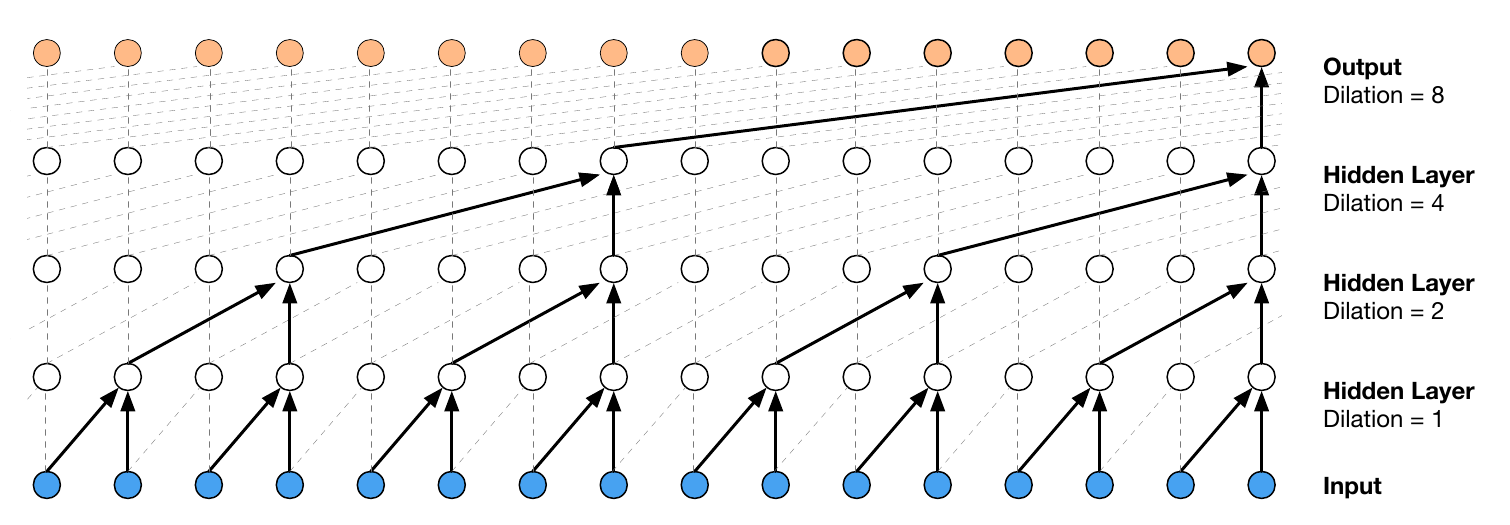
\includegraphics[scale=0.3]{img/casual_dilated}
Свёртки - главный ингредиент WaveNet. Используя свёртки, мы гарантируем, что модель не может нарушить первоначальный порядок данных: предсказание $p(x_{t+1} = x_1, \dots, x_{t})$, выдаваемое моделью в момент времени $t$ не может зависеть ни от каких моментов в будущем $x_{t+1}, x_{t+2}, \dots, x_{T}$. Вы это можете наблюдать на рисунке \ref{fig:casual}.

\label{sec:convolutions}

\begin{figure}[ht!]
    \centering
  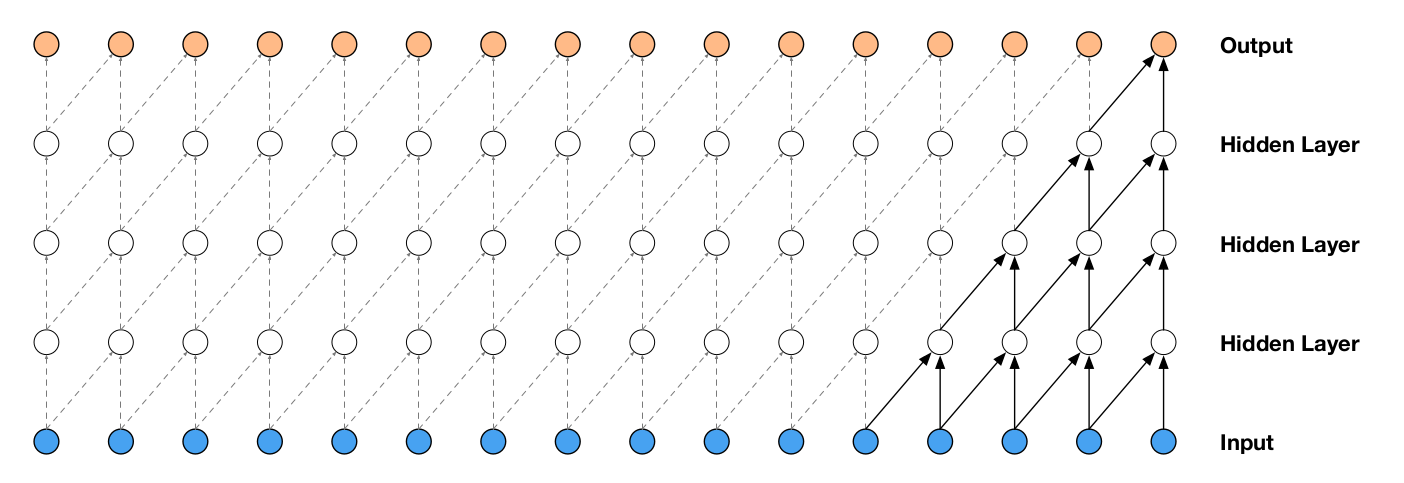
\includegraphics[scale=0.35]{img/casual}
  \caption{Рецептивное поле для стека свёрточных слоёв}
  \label{fig:casual}
\end{figure}

При обучении условные вероятности во все моменты времени могут вычисляться параллельно, потому что все значения сигнала $x$ заранее известны. Во время генерации предсказания последовательны: каждая предсказанная точка подаётся обратно на вход нейросети, чтобы предсказать следующую.

Поскольку модели со свёртками не имеют рекуррентных соединений, они обычно обучаются быстрее нежели рекуррентные архитектуры, особенно когда применяются к длинным последовательностям. Одна из проблем  свёрток заключается в том, что они требуют большого количества слоёв либо большие размеры фильтров, чтобы увеличить ширину рецептивного поля. Например, на рисунке \ref{fig:casual} ширина рецептивного поля равна 5 (=\#слоёв + длина фильтра - 1). Для решения этой проблемы и появились свёртки с дырками, позволяющие на порядки увеличить рецептивное поле, не накладывая больших вычислительных затрат. 

\newpage
\subsection{Дырявые свёртки}

Дырявые свёртки это свёртки, в которых фильтр применяется по диапазону больше своей длины, пропуская входные значения с некоторым шагом. Это эквивалентно свёртке с большим фильтром, "продырявленным" нулями, но значительно эффективнее вычислительно. Такая эффективность дырявых свёрток позволяет нейросети оперировать более крупными данными, нежели позволили бы обычные свёртки. В частном случае дырявые свёртки с пропуском 1 эквиваленты обычным свёрткам. На рисунке \ref{fig:casual_dilated} изображены дырявые свёртки с промежутками 1, 2, 4 и 8. 

\begin{figure}[h!]
  \centering
  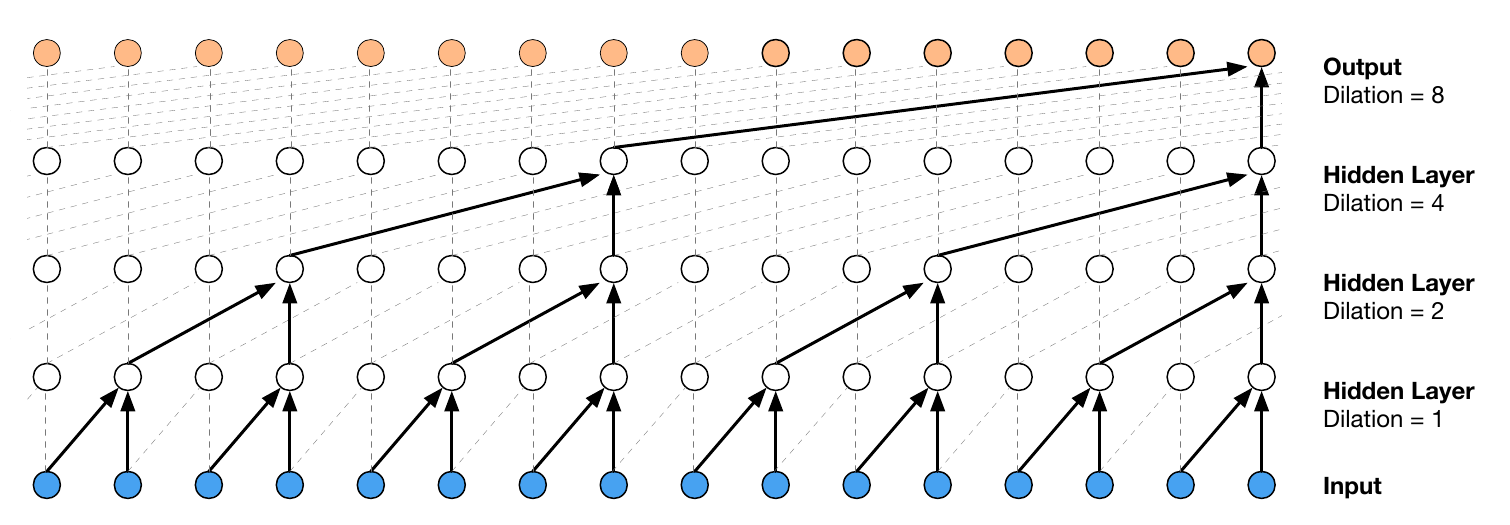
\includegraphics[scale=0.32]{img/casual_dilated}
  \caption{Рецептивное поле для стека дырявых свёрточных слоёв}
  \label{fig:casual_dilated}
\end{figure}

Стеки дырявых свёрток позволяют достичь очень широкого рецептивного окна с помощью небольшого количества слоёв, при этом сохраняя качество входных данных на протяжении всей сети. В оригинальном WaveNet промежутки увеличиваются в два раза для каждого слоя пока не достигнут какого-то фиксированного значения, и затем всё повторяется. Например:
$$1,2,4,\dots, 512, 1,2,4,\dots, 512, 1,2,4,\dots, 512.$$ 

Попробуем объяснить интуицию за такой конфигурацией. Во-первых, экспоненциальное увеличение промежутков приводит к экспоненциальному по глубине росту окна. \cite{arxiv:yu-fisher} Например, каждый $1,2,4, \dots 512$ блок имеет окно размера $1024$ его можно воспринимать в качестве более эффективной и имеющей большую описательную силу альтернативы свёртки $1 \times 1024$. Во-вторых, дальнейшее объединение таких слоёв в стеки увеличивает объём модели и ширину окна.

\newpage
\subsection{Gated activation unit}

\begin{definition}
\textbf{Gate} в контексте нейросетей это термин, мигрировавший из электрических сетей. Поскольку любые операции могут быть описаны в качестве графовых примитивов, gate в самом широком смысле можно назвать операцию любой арности. Одним из простейших примеров gate является умножение.

Ключевой gate в архитектуре называемый update gate находится на выходе из каждой пачки свёрточных слоёв.

\begin{figure}[ht!]
  \centering
  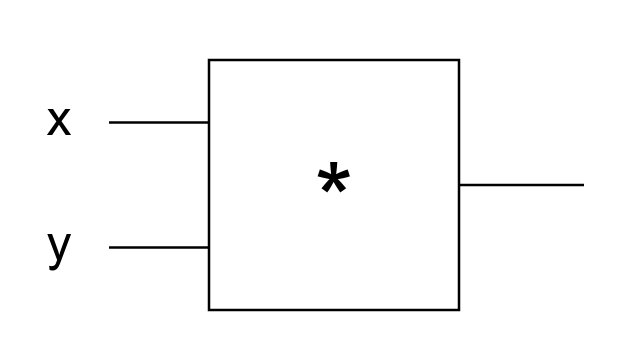
\includegraphics[scale=0.35]{img/gate}
  \caption{Простейший gate}
  \label{fig:gate}
\end{figure}

\end{definition}

Gated activation unit выглядит так:

\begin{equation} \label{eq:activation_func}
z = \tanh(W_{f,k} * x \  \astrosun \  \sigma(W_{g,k} * x))
\end{equation}


где $*$ обозначает операцию свёртки, $\astrosun$ обозначает поэлементное умножение, $\sigma(\cdot)$ сигмоида, $k$ номер слоя, $f$ и $g$ обозначают фильтр и gate соответственно, и $W$ обучаемый свёрточный фильтр. Авторы WaveNet утверждают, что такая функция активации работает значительно лучше для генерации аудиосигналов чем стандартная rectified linear activation function.

\newpage
\subsection{Residual и skip соединения}

\begin{figure}[ht!]
  \centering
  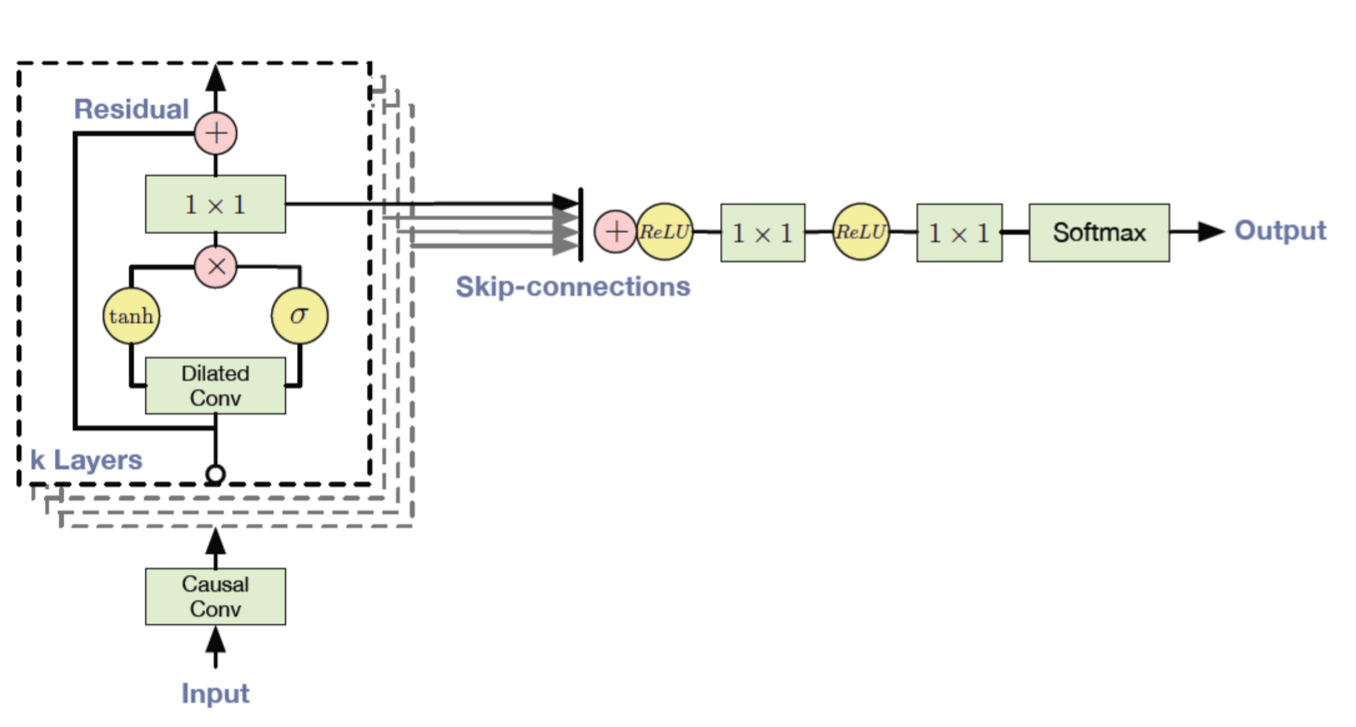
\includegraphics[scale=0.35]{img/wavenet}
  \caption{Архитектура WaveNet}
  \label{fig:wavenet_arch}
\end{figure}

\begin{definition}
\textbf{Skip} соединение в нейронной сети это соединение, которое пропускает слой и соединяется к следующему доступному слою. В общем случае может быть пропущен более чем один слой.
\end{definition}

\begin{definition}
\textbf{Residual} соединение присоединяется к предыдущему слою.
\end{definition}

В архитектуре используются residual и параметрические skip соединения, чтобы ускорить сходимость и позволить обучение более глубоких моделей. На рисунке \label{fig:wavenet_arch} виден residual блок модели, который повторяется много раз в архитектуре. 

\newpage
\end{document}

